\documentclass[a4paper,norsk]{article}
\usepackage[latin1]{inputenc}
\usepackage[T1]{fontenc}
\usepackage{babel,textcomp,listings, subfigure,graphicx}
\usepackage{subfig}

                                    
\title{Assignment 1, Mek4250}
\author{Sebastian Gjertsen}
\begin{document}
\maketitle
\section*{1}
\subsection*{a)}
The $H^p$ norm consist of the L2 norm plus all the derivatives up the hth degree.
$$ \vert \vert u \vert \vert_1 = \big( \int u^2 + \frac{\partial u}{\partial x}^2\big)^\frac{1}{2} = sin(\pi kx)^2 cos(\pi ly)^2  +  (\pi k cos(\pi kx)cos(\pi ly) - \pi l sin(\pi kx)sin(\pi ly))^2$$
$$ \vert \vert u \vert \vert_1 = \big( \pi^2 (k^2+l^2)(\frac{1}{4}) \big) ^\frac{1}{2}$$ 
We get this recurring for every added degree of h. Giving:

$$ \vert \vert u \vert \vert_h = \big(\sum_i^h  \pi^{2i} (k^2+l^2)^i\big)^\frac{1}{2} \hspace{1mm} ( \frac{1}{2})$$





\subsection*{b)}
To compute the H1 and L2 norms i used the norms from FENiCS. As can be seen in the code in the bottom of this section.
We can see from the tables of errornorms that the error gets smaller with increasing number of elements and the error increases when we have more oscillations of the sine and cosine functions. The first part makes sense since we can more accurately represent the functions with more points in the mesh. And the latter makes sense because with more oscillations than elements in one direction we only get sort of parts of the function as in crosses through the element. This is in general for the error. \newline
For the H1 norm the errornorm gets bigger when we increase k and l because the derivative is gets higher for steeper functions.

\begin{lstlisting}
LAGRANGE = 1

L2 NORM
N / k&l  1           10              100
8        0.0328      0.6775     159.9224
16      0.0085      0.3634      247.3597
32      0.0021      0.1779      2.5068
64      0.0005      0.0549      3.6142

H1 NORM
N / k&l  1               10                       100
8       0.43611616   25.51151631    3232.51360546
16      0.21810459   17.23357873    4689.64045220
32      0.10904725   10.54385048    450.33238520
64      0.05452270   5.43087909     534.88053004



LAGRANGE = 2

L2 NORM
N / k&l  1                10                   100
8       0.00056880    0.42444612   293.08481819
16      0.00006933    0.08864854   90.52742877
32      0.00000861    0.01017424   4.57194541
64      0.00000108    0.00113884   1.47234385


H1 NORM
N / k&l  1                 10                    100
8       0.03314086    17.66688309   5315.73621535
16      0.00838664    6.71715133    1657.67783190
32      0.00210537    1.96195378    702.19909726
64      0.00052716    0.51734696    270.00322078
\end{lstlisting}


\subsection*{c)}
I used the norms  
 $$ \vert \vert u-u_h \vert \vert_{0} \leq C h^\alpha \vert \vert u \vert \vert_{1} $$
 $$ \vert \vert u-u_h \vert \vert_{1} \leq C h^\alpha \vert \vert u \vert \vert_{2} $$
I did this exercise before the assignment was changed, and it does not change that value of the alpha if we have the norm of u on the LHS. The C will change a bit but we are only looking at if C is big or small not some exact value. \newline
To compute $C$ and $\alpha$ I used the least squares from numpy and made my own, as you can see in the code, to check that it was correct. With lagrange = 1,  L2 and H1 norms, k and l 1 and 10 I got  $\alpha \approx 2$ and with k and l 100 is almost 3. The C gets high as we increase k and l.  \newline
It seems in general that L2 and H1 norms produce better $(\alpha=2)$ and $C = high$ \newline
We can see in figure 1 and 2 that the least squares interpolates the best line over the points calculated for different N values. When k gets higher it is harder to find a suitable line and therefore our $\alpha$ and C values are gets worse. 



\begin{lstlisting}

LAGRANGE = 1

L2 and H1 norms:

k = l     C               alpha
1         0.304057859582  1.82285696122
10        9.51367285062   2.25838702398
100       23111.6349906   3.24004809894

H1 and H2 norms:
k = l     C                alpha
1         0.371924037408   1.9111252817
10        0.221516452868   1.11933011599
100       0.397735012462   1.03231000867

LAGRANGE = 2

L2 and H1 norms:

k = l     C                alpha
1         0.151996496825  3.73753264544
10        18.7979921884   3.31590714197
100       1864.5698256    2.81857174656

H1 and H2 norms:
k = l     C                 alpha
1          0.0975858435078  2.59587384003
10         0.632411889525   2.04983515805
100       0.191004437667   0.915842115932
\end{lstlisting}

\begin{figure}[h]
    \centering
    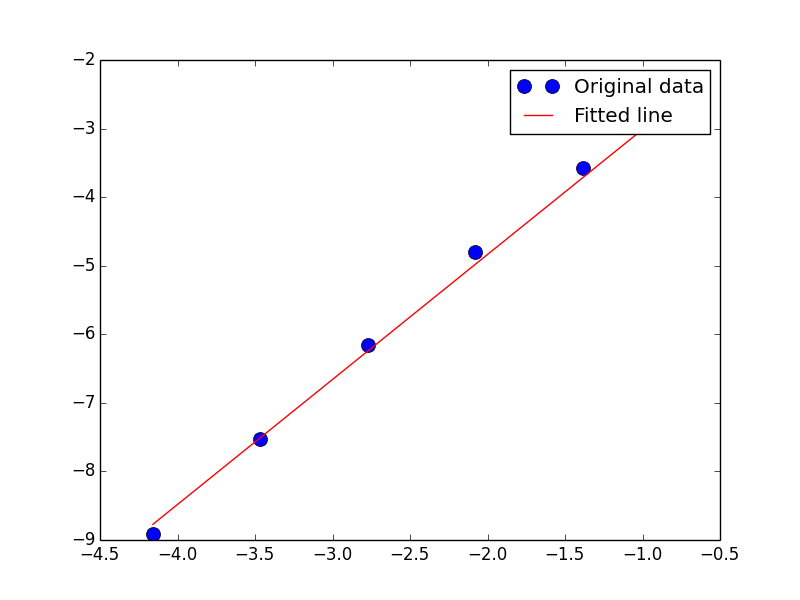
\includegraphics[scale=0.5]{least_squares_1_1.png}
    \caption{Least Squares, k = l = 1 , polynomial = 1}
    \label{fig:awesome_image}
    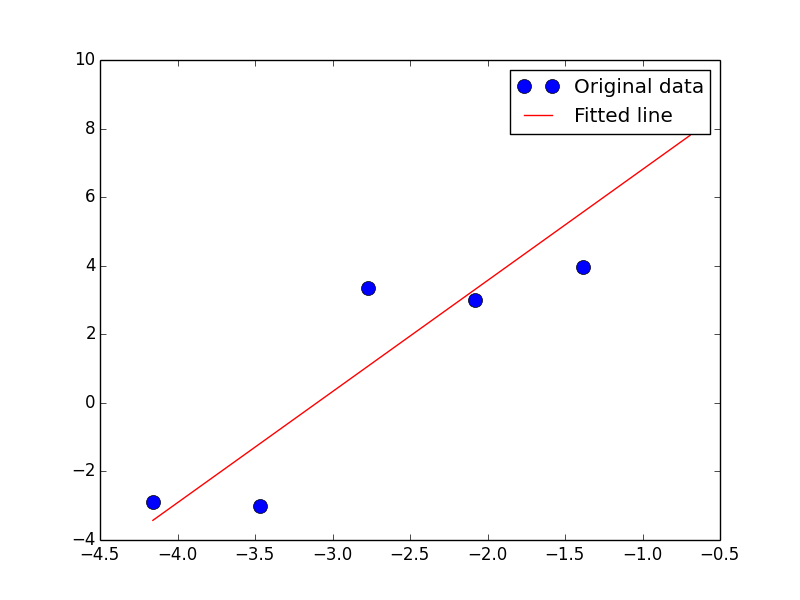
\includegraphics[scale=0.5]{least_squares_1_100.png}
    \caption{Least Squares, k = l = 100, polynomial = 1}
    \label{fig:awesome_image}
\end{figure}





\subsection*{Code}
\lstinputlisting[language=Python]{Ex_1.py}

\newpage

\section*{2}
\subsection*{a)}
To solve this equation analytically we use the method separation of variables and say that $u(x,y) = U(x)*V(y)$\newline
We insert this solution into the equation and get:
$$ \mu \frac{V_{yy}}{V} = \mu \frac{U_{xx}+ U_x}{U}  = \lambda$$
The LHS we know has the solution $V = C_1 sin((\frac{\lambda}{\mu})^{\frac{1}{2}}y)+ C_2 cos((\frac{\lambda}{\mu})^{\frac{1}{2}}y)$ and a solution to this equation is when $\lambda = 0$, giving $Y = 1$
This upholds the boundary conditions in y-direction.
\newline
The RHS has the known solution, with $\lambda = 0$:
$$U = \frac{e^{\frac{x}{\mu}-1}}{e^{\frac{1}{\mu}-1}}$$
This upholds the boundary condition in x-direction.
Giving then:
$$u(x,y) = \frac{e^{\frac{x}{\mu}}-1}{e{\frac{1}{\mu}-1}}$$


\subsection*{b)}

\begin{lstlisting}

LAGRANGE ELEMENTS = 2

L2 - NORM:


mu = 1e+00 , N = 8 Numerical Error: 1.1511e-05

mu = 1e+00 , N = 16 Numerical Error: 1.4484e-06

mu = 1e+00 , N = 32 Numerical Error: 1.8175e-07

mu = 1e+00 , N = 64 Numerical Error: 2.2766e-08

mu = 1e-01 , N = 8 Numerical Error: 2.2325e-03

mu = 1e-01 , N = 16 Numerical Error: 3.0338e-04

mu = 1e-01 , N = 32 Numerical Error: 3.8830e-05

mu = 1e-01 , N = 64 Numerical Error: 4.8872e-06

mu = 1e-02 , N = 8 Numerical Error: 7.6887e-02

mu = 1e-02 , N = 16 Numerical Error: 2.7731e-02

mu = 1e-02 , N = 32 Numerical Error: 7.3478e-03

mu = 1e-02 , N = 64 Numerical Error: 1.3145e-03

mu = 1e-03 , N = 8 Numerical Error: nan

mu = 1e-03 , N = 16 Numerical Error: nan

mu = 1e-03 , N = 32 Numerical Error: nan

mu = 1e-03 , N = 64 Numerical Error: nan

\end{lstlisting}
We see that the error goes down with increasing number of elements and with decreasing $\mu$. When we decrease the mu past 0.001, python cannot represent that exponential. Thats why we get nan.

\subsection*{c)}

To calculate the C and $\alpha$ i used the norms 
 $$ \vert \vert u-u_h \vert \vert_{0} \leq C h^\alpha  $$
 $$ \vert \vert u-u_h \vert \vert_{1} \leq C h^\alpha  $$

\begin{lstlisting}
LAGRANGE ELEMENTS = 1
L2 and H1

mu =  1.0 C =   0.077217550709 alpha =   1.99848415122
mu =  0.1 C =   0.559578704657 alpha =   1.9343298292
mu =  0.01 C =   2.78391620437 alpha =   1.83179131516


LAGRANGE ELEMENTS = 2
L2 and H1

mu =  1.0  C =   0.00494279949017 alpha =   2.98835482613
mu =  0.1  C =   0.246231900242   alpha =   2.75535616309
mu =  0.01 C =   1.07890852871    alpha =   2.04562047668

\end{lstlisting}
We expected from theory that $\alpha \approx $  (element degree)  $ +1$.\newline
Which is what we find. When the elements have degree 1 the alpha becomes 2 with L2 and H1 norm. And likewise for higher elements.
\begin{lstlisting}

LAGRANGE ELEMENTS = 1 
H1 norm
mu =  1.0 C =   0.298768477069 alpha =   0.998517422902
mu =  0.1 C =   4.01201969534 alpha =   0.861879498393
mu =  0.01 C =   15.4545207055 alpha =   0.378727137865

LAGRANGE ELEMENTS = 2
H1 norm
mu =  1.0 C =   0.0365363825599 alpha =   1.9838208629
mu =  0.1 C =   3.83850565709 alpha =   1.77422820512
mu =  0.01 C =   18.2184701683 alpha =   0.738632714997
\end{lstlisting}

When we changed to the H1 error norm we expected to get alpha the same as the degree of elements. This is what we get and like before it gets worse as we lower $\mu$


\subsection*{d)}

To compute the SUPG i just changed the test function to  $v = v + beta * mesh.hmin() * v.dx(0)$. This method will smooth out our solution giving us a better solution when dealing with sharp corners. We see, from the table under, that the error is a $10^{-1}$ bigger than for Galerkin in the lower case. Putting beta lower gets us closer to Galerkin method so its expected that the error will be better for smaller beta.\newline
SUPG can be a useful tool when we have a very sharp edge that we have a problem computing, since it smooths out the solution. Not giving a perfect answer but at least being able to compute over the domain.\newline
We see from figure 3 that Galerkin with small $\mu$ gives oscillations and a bad solution. And figure 4 with SUPG gives a smoother and better solution.\newline
To compute the C and alpha in the error estimates I implemented the SUPG errornorm (6.8) from the compendium. And was looking to get alpha = degree$*\frac{3}{2}$. I implemented the errornorm the following way:
\begin{lstlisting}
    ex_norm = assemble((u_exact.dx(0) - u.dx(0))**2*dx)
    ey_norm = assemble((u_exact.dx(1) - u.dx(1))**2*dx)
    e = sqrt(mesh.hmin()*ex_norm + mu*(ex_norm+ey_norm))
\end{lstlisting}
A print of this norm with varying $\mu$ and $h$

\begin{lstlisting}
beta = h.min()
SUPG - norm

h/mu    1.0                0.1             0.01
2       0.231884809424     1.37374796004   1.48337689453
4       0.119830544311     1.04782853084   1.53689283747
8       0.0611456253743    0.667343103029  1.56955648944
16      0.0309330012785    0.385035688553  1.51741616324
32      0.0155652178542    0.209127121281  1.2126647182
64      0.00780854650798   0.109434586932  0.795300364213


mu =  1.0   C =   0.330129747596  alpha =   0.979369968414
mu =  0.1   C =   2.11805769892   alpha =   0.743376329069
mu =  0.01  C =   1.83477492663   alpha =   0.159166143481


beta = h.min()
L2 - norm

h/mu     1.0                0.1             0.01
2        0.0487459798451    0.365048142768  0.395142264119
4        0.0265760049303    0.286879143016  0.348635524567
8        0.0141685886099    0.192691162916  0.266450466069
16       0.0073698766431    0.114521156974  0.189592045188
32       0.00376694891544   0.0628907014983 0.125314777253 
64       0.00190550308829   0.0330610795148 0.0769559179375

mu =  1.0   C =   0.0697885911129   alpha =   0.936689949943
mu =  0.1   C =   0.561676604788    alpha =   0.704104417791
mu =  0.01  C =   0.544386376465    alpha =   0.47773708412

\end{lstlisting}
I was expecting to see $\alpha =1.5$ from the SUPG norm. \newline
We can see from the L2 errornorm estimate that that our $\alpha$ is not where it was with Galerkin. This points to the fact that SUPG is not as accurate.
\begin{lstlisting}


LAGRANGE ELEMENTS = 2
L2 NORM:
beta = h.min()*1.0

mu = 1e+00 , N = 8 Numerical Error: 1.2625e+00
mu = 1e+00 , N = 16 Numerical Error: 3.4611e-01
mu = 1e+00 , N = 32 Numerical Error: 3.3307e+00
mu = 1e+00 , N = 64 Numerical Error: 2.4616e+03

mu = 1e-01 , N = 8 Numerical Error: 2.4907e-01
mu = 1e-01 , N = 16 Numerical Error: 1.5145e-01
mu = 1e-01 , N = 32 Numerical Error: 5.2001e+00
mu = 1e-01 , N = 64 Numerical Error: 1.0097e+04

mu = 1e-02 , N = 8 Numerical Error: 2.7716e-01
mu = 1e-02 , N = 16 Numerical Error: 1.9793e-01
mu = 1e-02 , N = 32 Numerical Error: 1.3499e-01
mu = 1e-02 , N = 64 Numerical Error: 5.0506e+03


LAGRANGE ELEMENTS = 2
L2 NORM:
beta = h.min()*0.15

mu = 1e+00 , N = 8 Numerical Error: 3.0109e-02
mu = 1e+00 , N = 16 Numerical Error: 1.5232e-02
mu = 1e+00 , N = 32 Numerical Error: 7.6622e-03
mu = 1e+00 , N = 64 Numerical Error: 3.8428e-03

mu = 1e-01 , N = 8 Numerical Error: 5.7559e-02
mu = 1e-01 , N = 16 Numerical Error: 3.0749e-02
mu = 1e-01 , N = 32 Numerical Error: 1.5944e-02
mu = 1e-01 , N = 64 Numerical Error: 8.1258e-03

mu = 1e-02 , N = 8 Numerical Error: 7.8816e-02
mu = 1e-02 , N = 16 Numerical Error: 5.9183e-02
mu = 1e-02 , N = 32 Numerical Error: 3.8149e-02
mu = 1e-02 , N = 64 Numerical Error: 2.2061e-02


\end{lstlisting}


\begin{figure}[h]
    \centering
    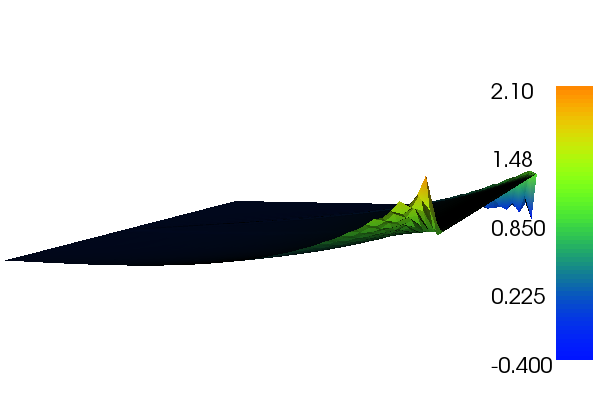
\includegraphics[scale=0.5]{dolfin_plot_3.png}
    \caption{Galerkin with $\mu = 0.0001$, N = 64}
    \label{fig:awesome_image}
    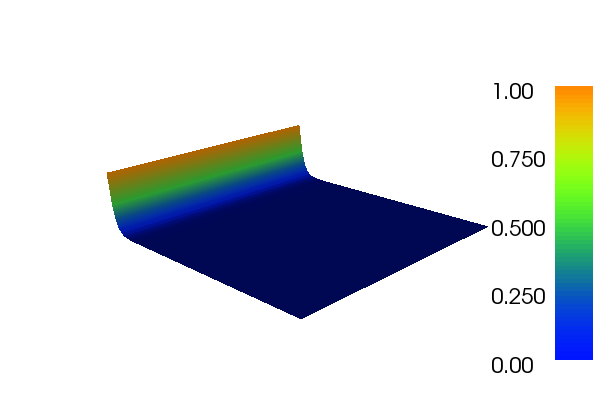
\includegraphics[scale=0.5]{dolfin_plot_0.png}
    \caption{SUPG with $\mu = 0.0001$, N = 64}
    \label{fig:awesome_image}
\end{figure}


\subsection*{Code}

\lstinputlisting[language=Python]{Ex_2.py}



















\end{document}